\chapter{HASIL DAN ANALISIS}

\section{Sub Bab Hasil}
\noindent Bab ini memaparkan pekerjaan penelitian dan, terutama, hasil-hasilnya, untuk dianalisis. Secara komprehensif bab ini merepre-sentasikan curahan pemikiran dan kemampuan mahasiswa dalam menjalani pekerjaan penelitian, yang hasil-hasilnya dapat dipertanggungjawabkan. Banyak pendukung yang diperlukan dalam penulisan bab ini, seperti skema penting pengolahan data, penurunan model matematika, asumsi khusus, tabulasi hasil dan analisis, dan gambar atau grafik yang membantu dalam paparan analisis. Judul bab dan sub bab disesuaikan dengan isi paparan.

\section{Memasukkan Gambar}
\noindent Setiap gambar harus dirujuk pada naskah TA, termasuk gambar pada Lam- piran, menggunakan huruf pertama kapital (G) dan nomor gambar, tidak berdasarkan posisi relatifnya (misalnya di bawah ini atau sebelum ini). Format gambar yang umum adalah jpg, png, dan postscript (ps atau eps). Ukuran huruf pada nama sumbu dan label gambar/grafik harus cukup besar dan jelas, demikian halnya dengan angka pada sumbu. Gambar dan grafik dapat berwarna dengan pilihan warna yang tegas dan jelas.

\subsection{Contoh Gambar Sederhana}
Contoh menginput gambar pada buku TA pada
\begin{figure}[h] %h artinya here!
\centering
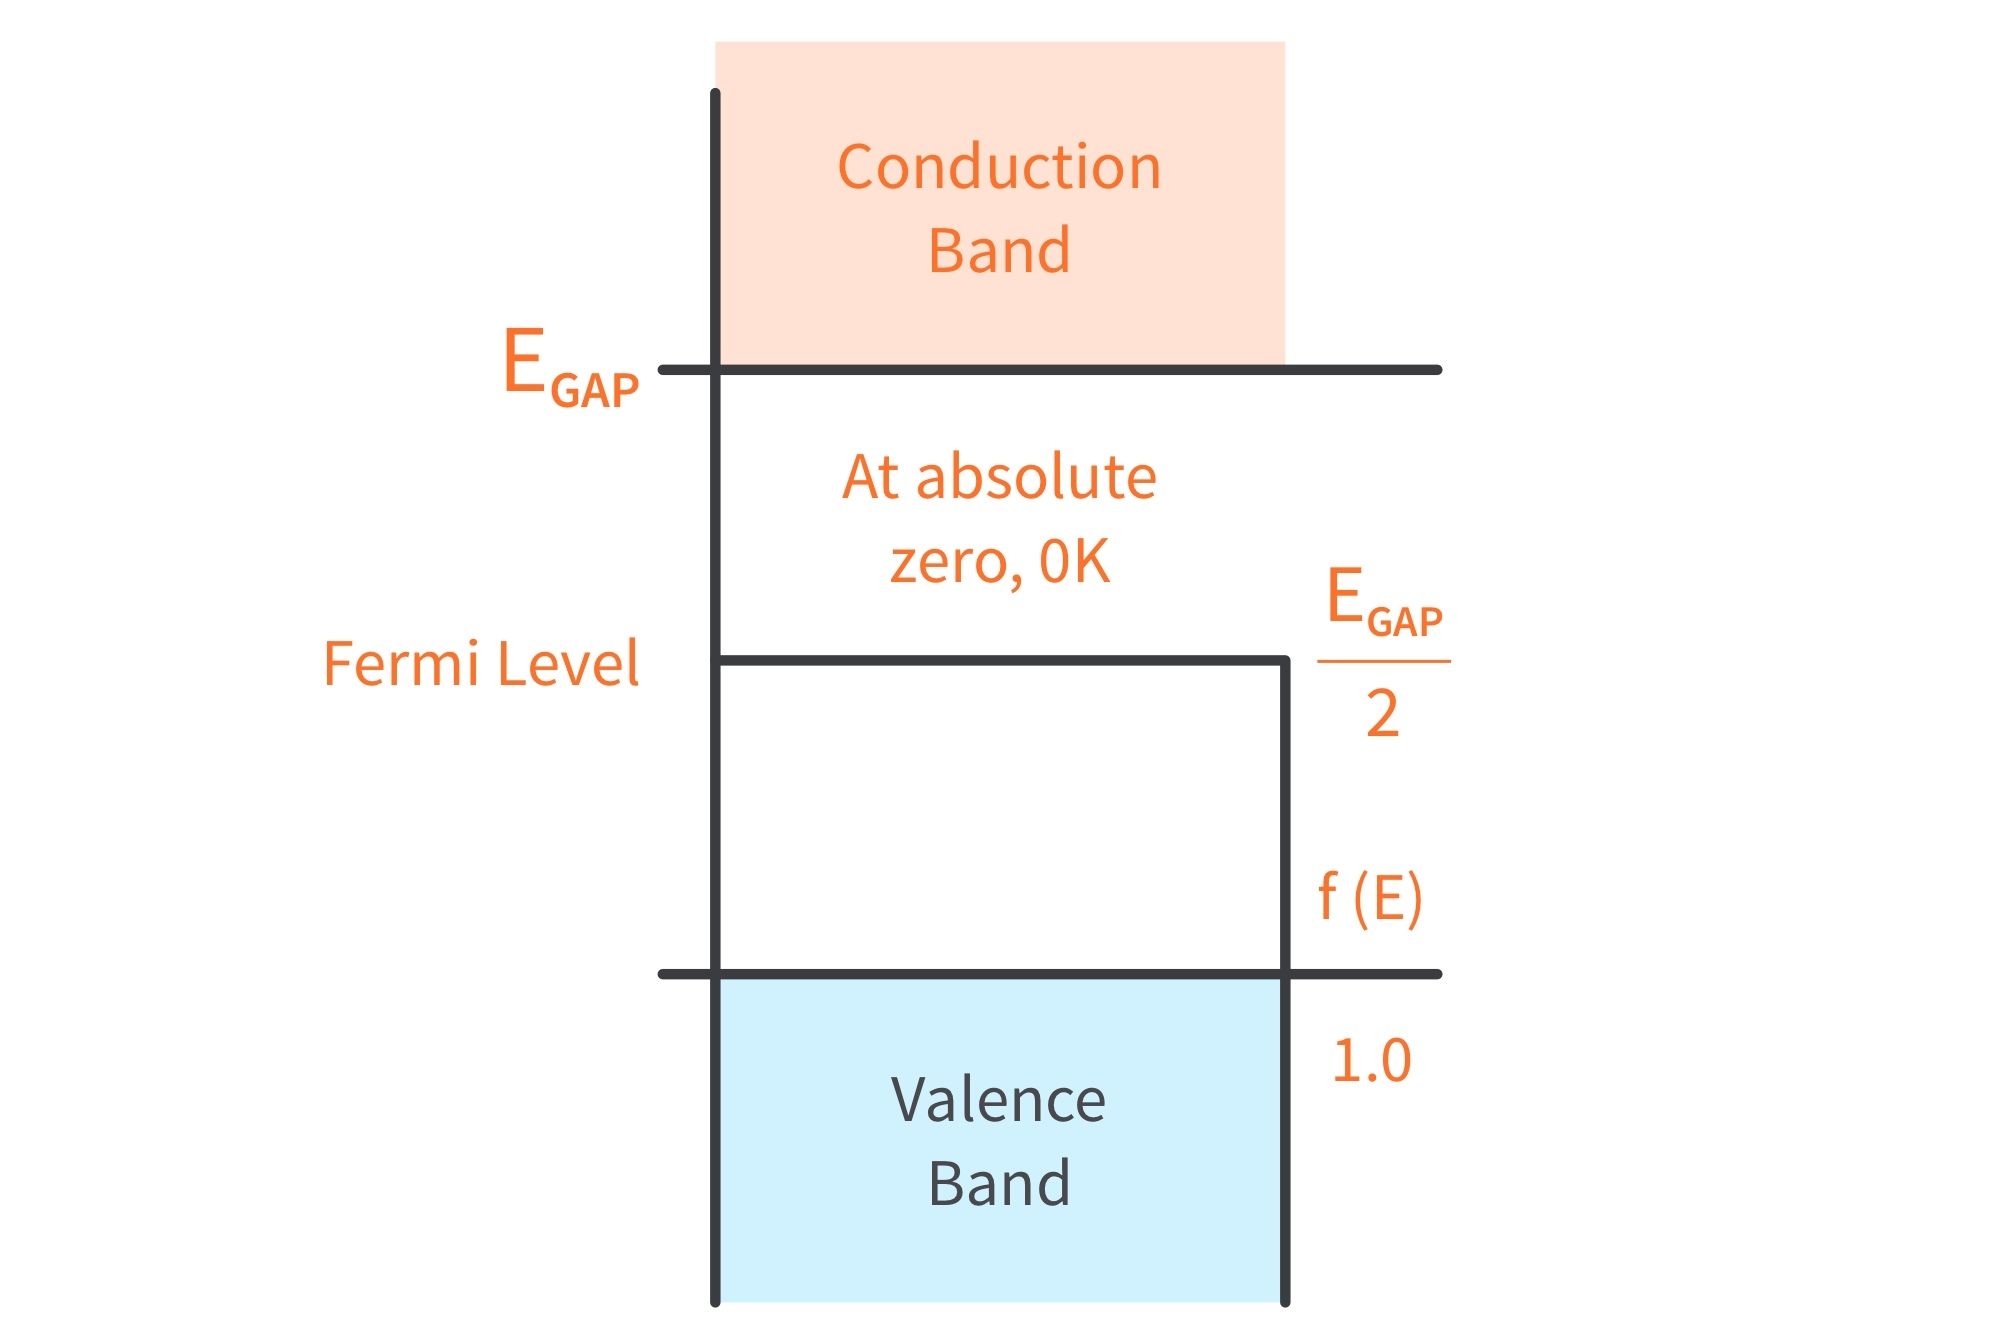
\includegraphics[width=0.3\linewidth]{gambar/Semiconductor-Fermi-Level-Band-Diagram-1.jpg}
\caption{Tingkatan Fermi pada\\Bahan Semikonduktor}
\label{fermilevel}
\end{figure}
Apabila ada dua gambar, kita juga bisa menaruh keduanya berdampingan.

\begin{figure}[H]
\centering
\subfigure[]{
 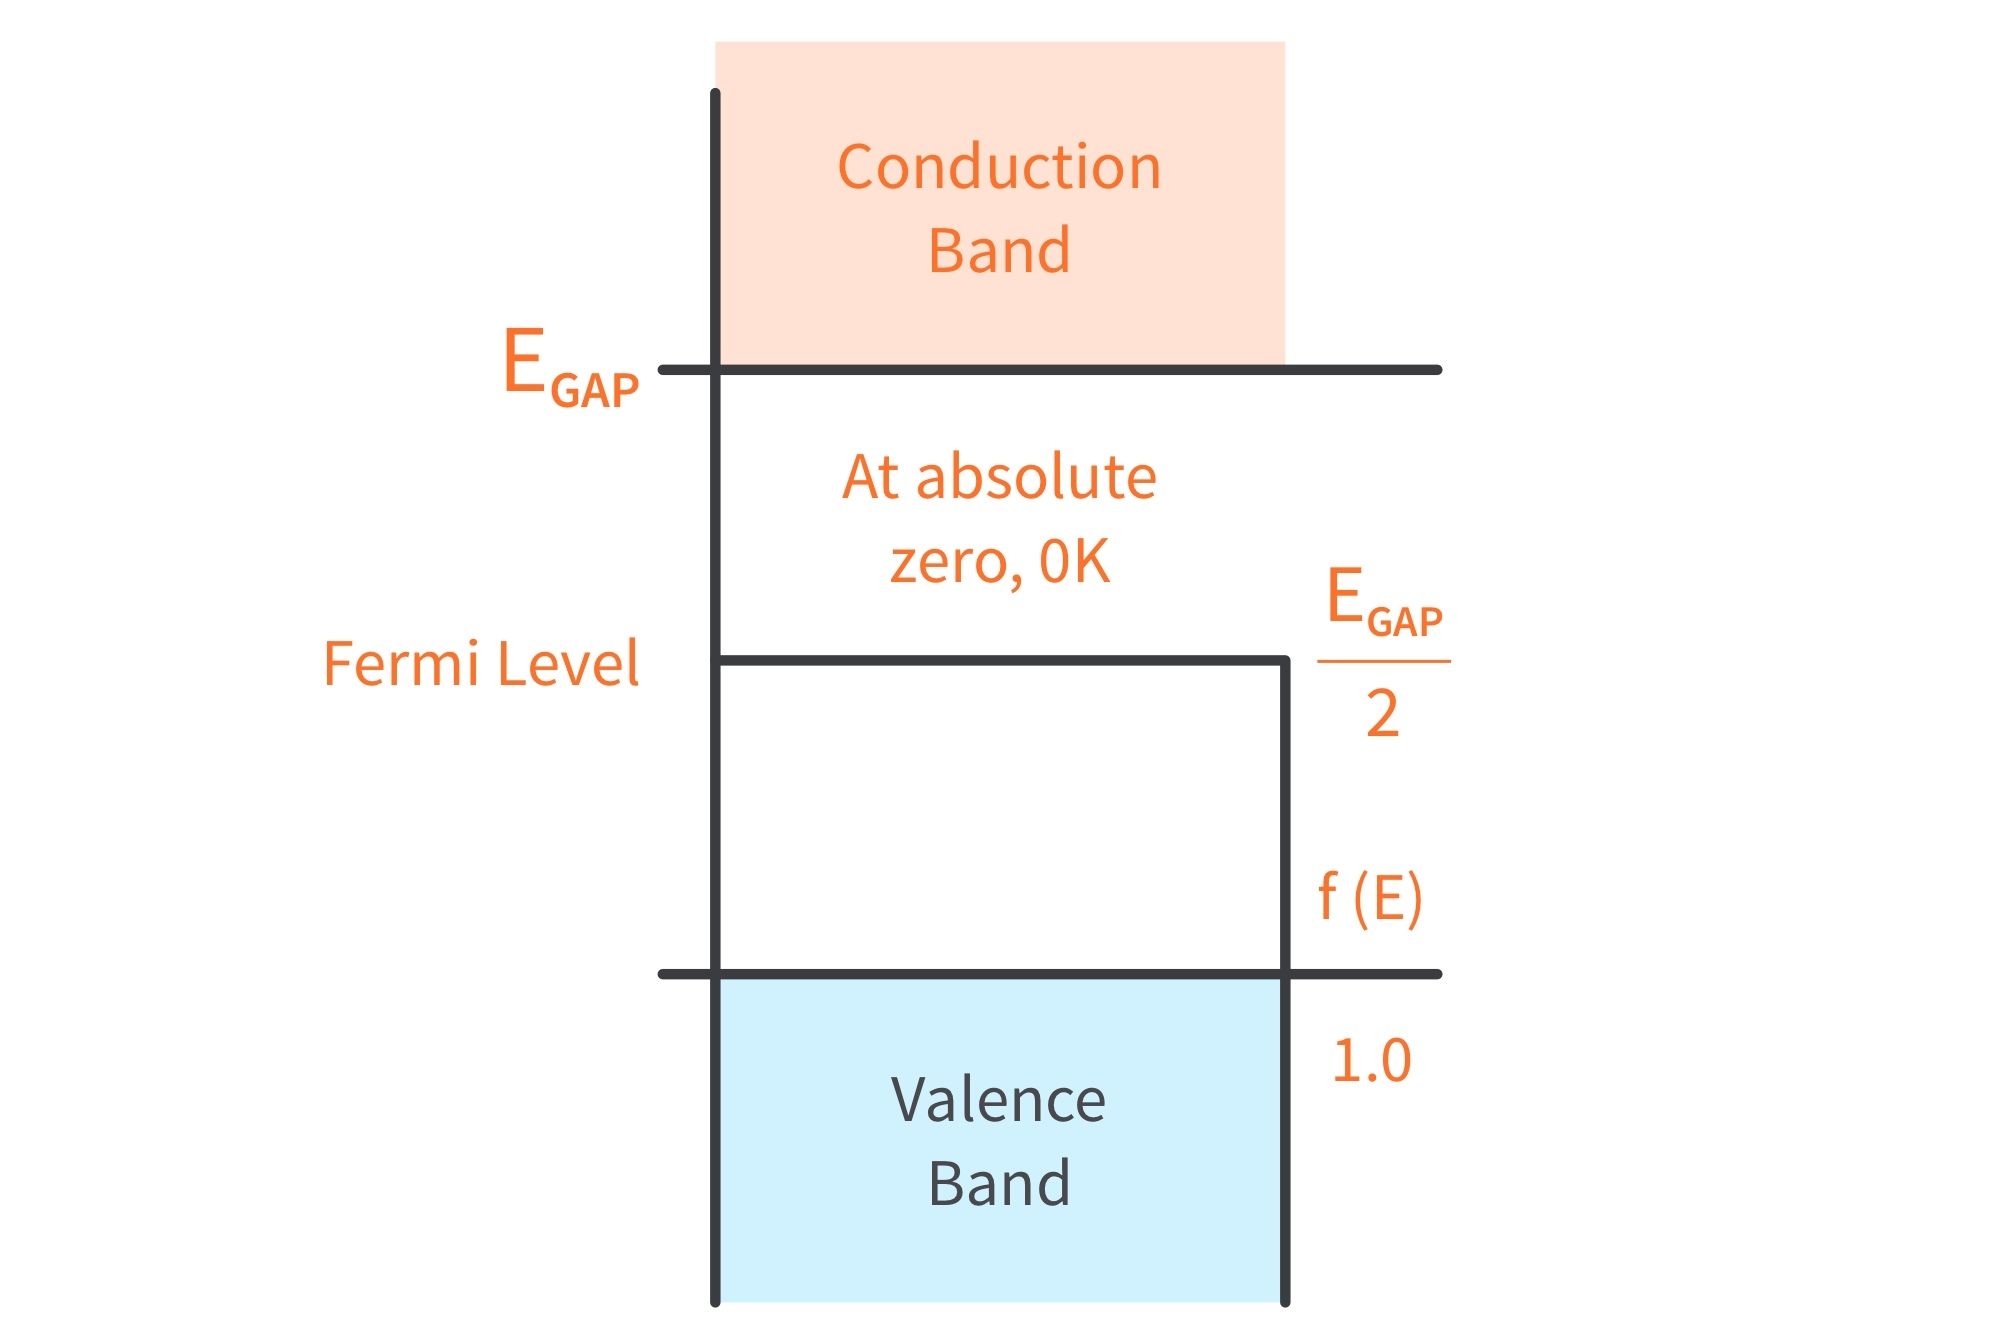
\includegraphics[width=0.4\linewidth]{gambar/Semiconductor-Fermi-Level-Band-Diagram-1.jpg}
 \label{surf-1}
 }\hspace{0.1\linewidth}
\subfigure[]{
 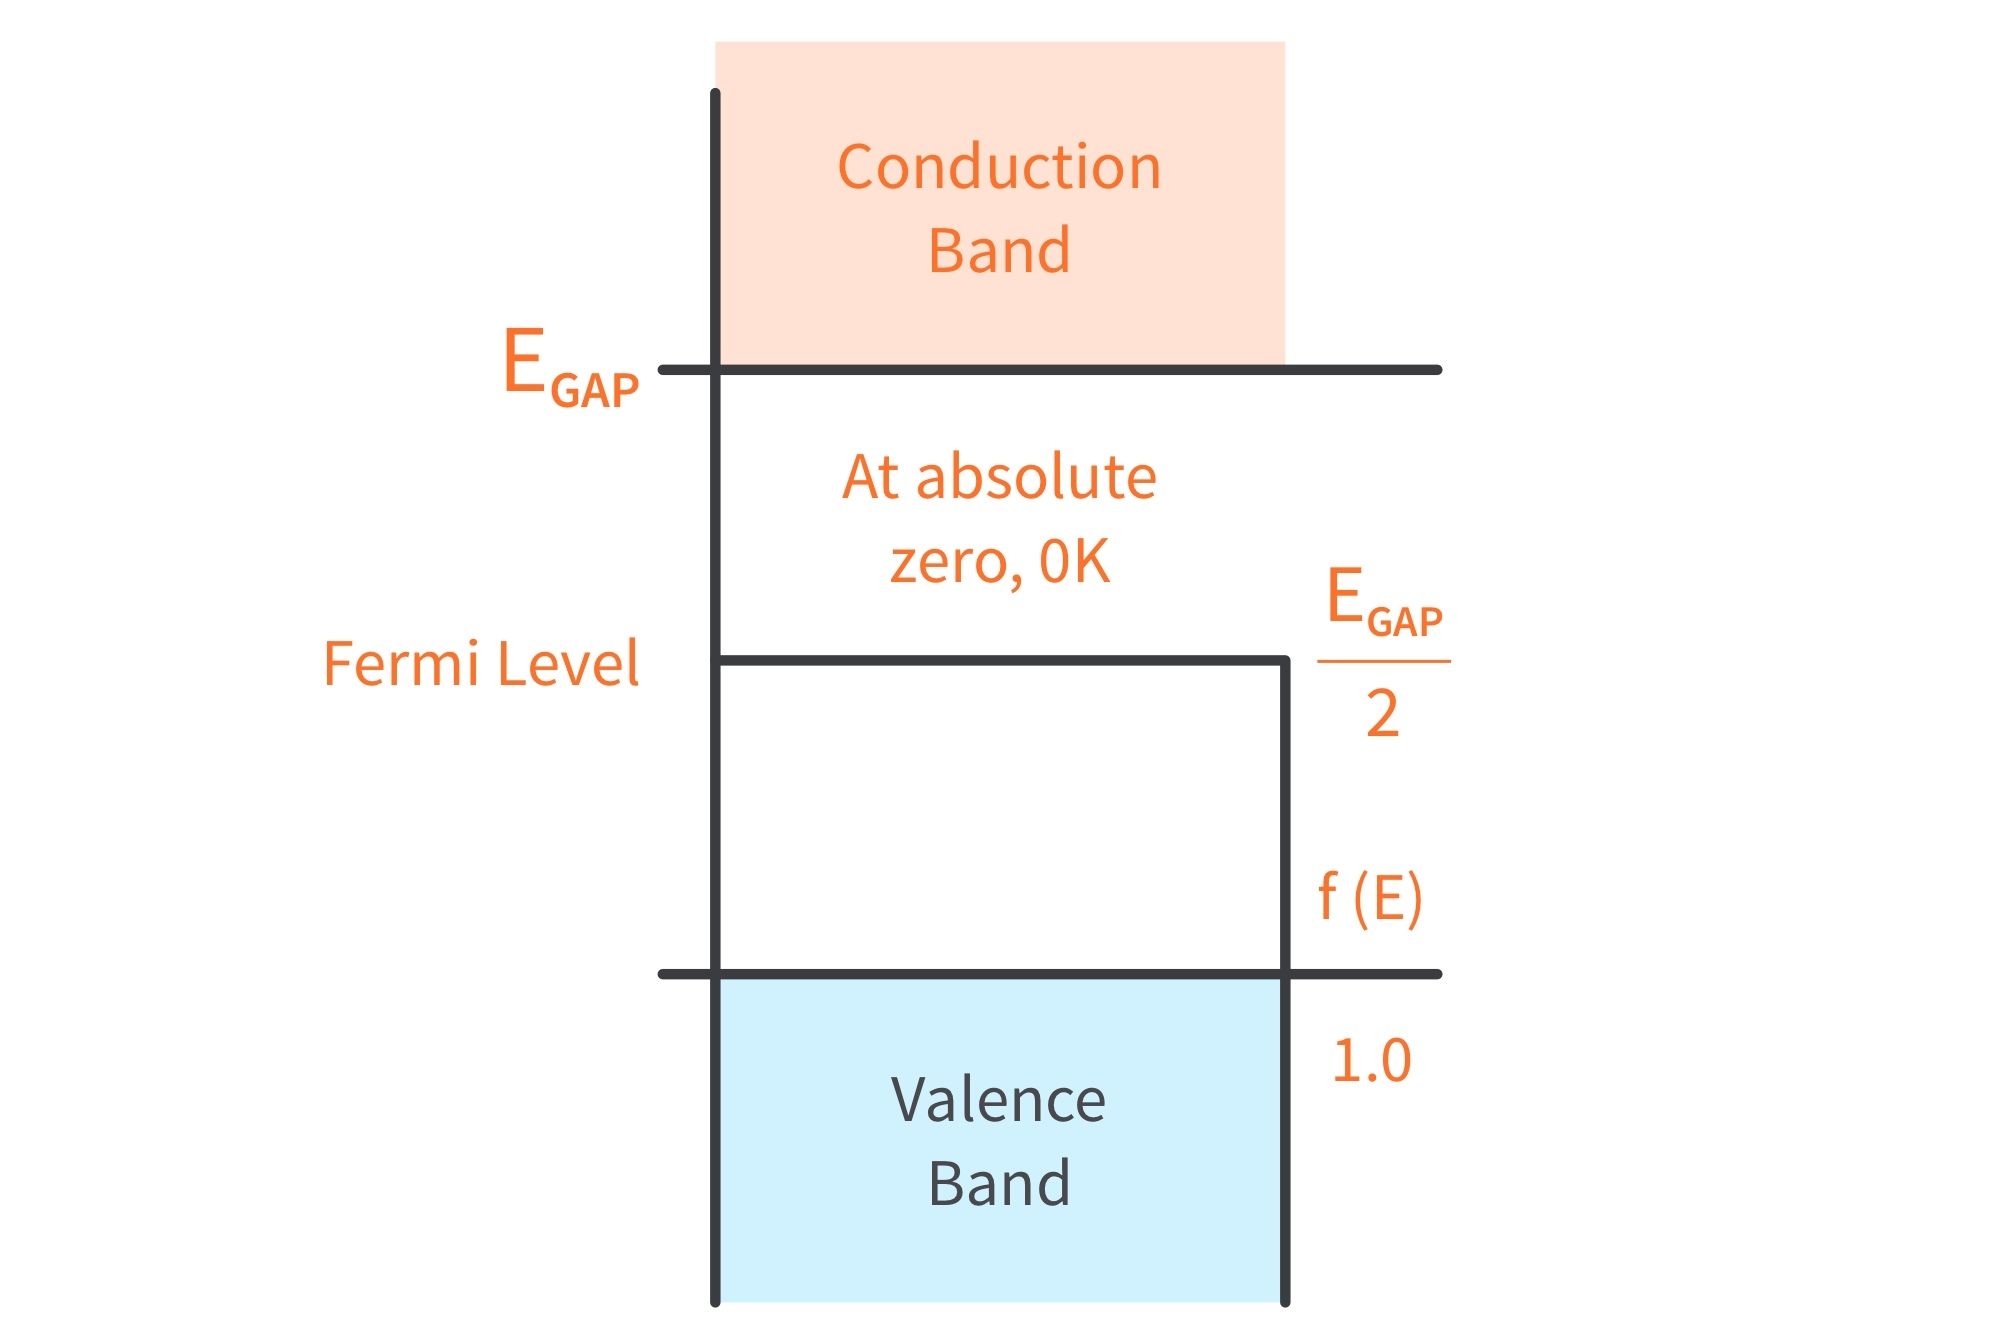
\includegraphics[width=0.4\linewidth]{gambar/Semiconductor-Fermi-Level-Band-Diagram-1.jpg}
 \label{surf-2}
}
\caption{Dengan menempatkan gambar \subref{surf-1} dan \subref{surf-2}, pembaca akan lebih mudah membandingkan keduanya.}
\label{surface}
\end{figure}